\chapter{Spanning Tree Protocol: Part
1}\label{spanning-tree-protocol-part-1}

\section{Redundancy in Networks}\label{redundancy-in-networks}

\begin{itemize}
\tightlist
\item
  Essential in network design
\item
  Modern networks are expected to run 24/7/265; even a short downtime
  can be disastrous for business.
\item
  If one network component fails, you must ensure that other components
  will take over with little or no downtime.
\item
  As much as possible, you must implement REDUNDANCY at every possible
  point in the network
\end{itemize}

\section{An Example of a Poorly Designed
Network}\label{an-example-of-a-poorly-designed-network}

\begin{figure}
\centering
\pandocbounded{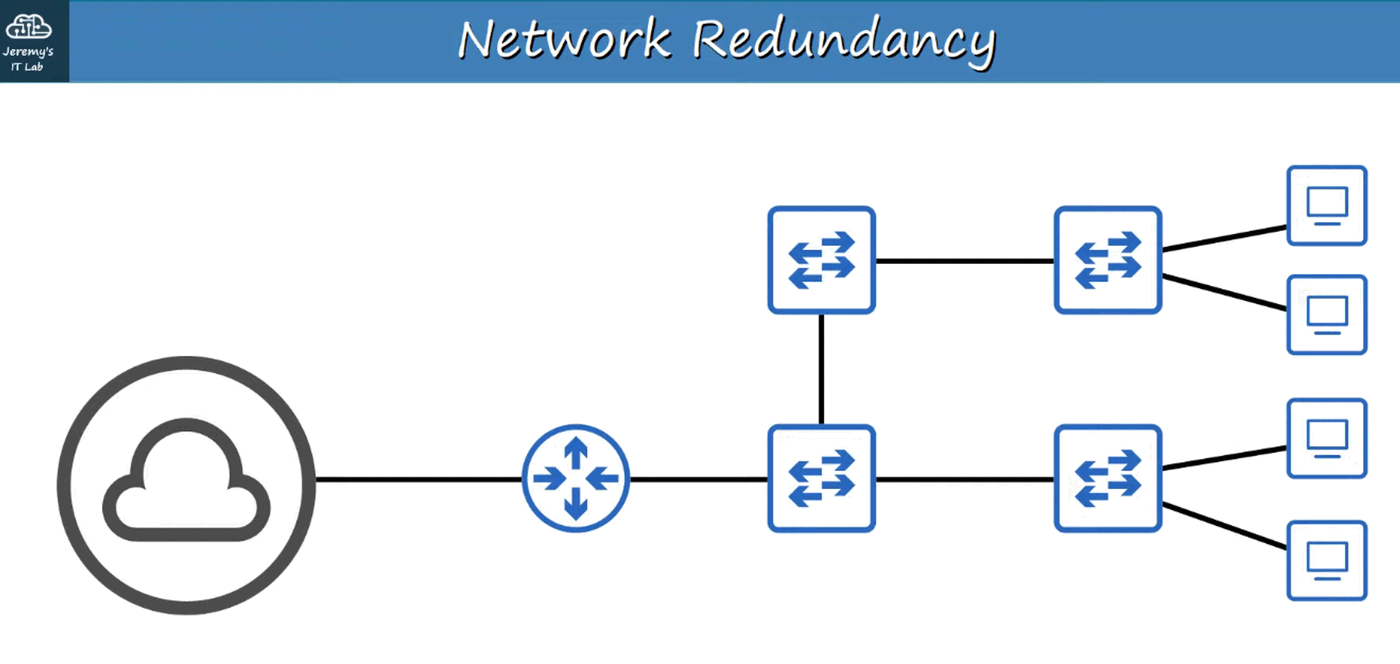
\includegraphics[keepaspectratio,alt={image}]{images/21-spanning-tree-protocol-part1/img-001.png}}
\end{figure}

NOTE the many single-point failures that could occur (single
connections)

\section{A Better Network Design}\label{a-better-network-design}

\begin{figure}
\centering
\pandocbounded{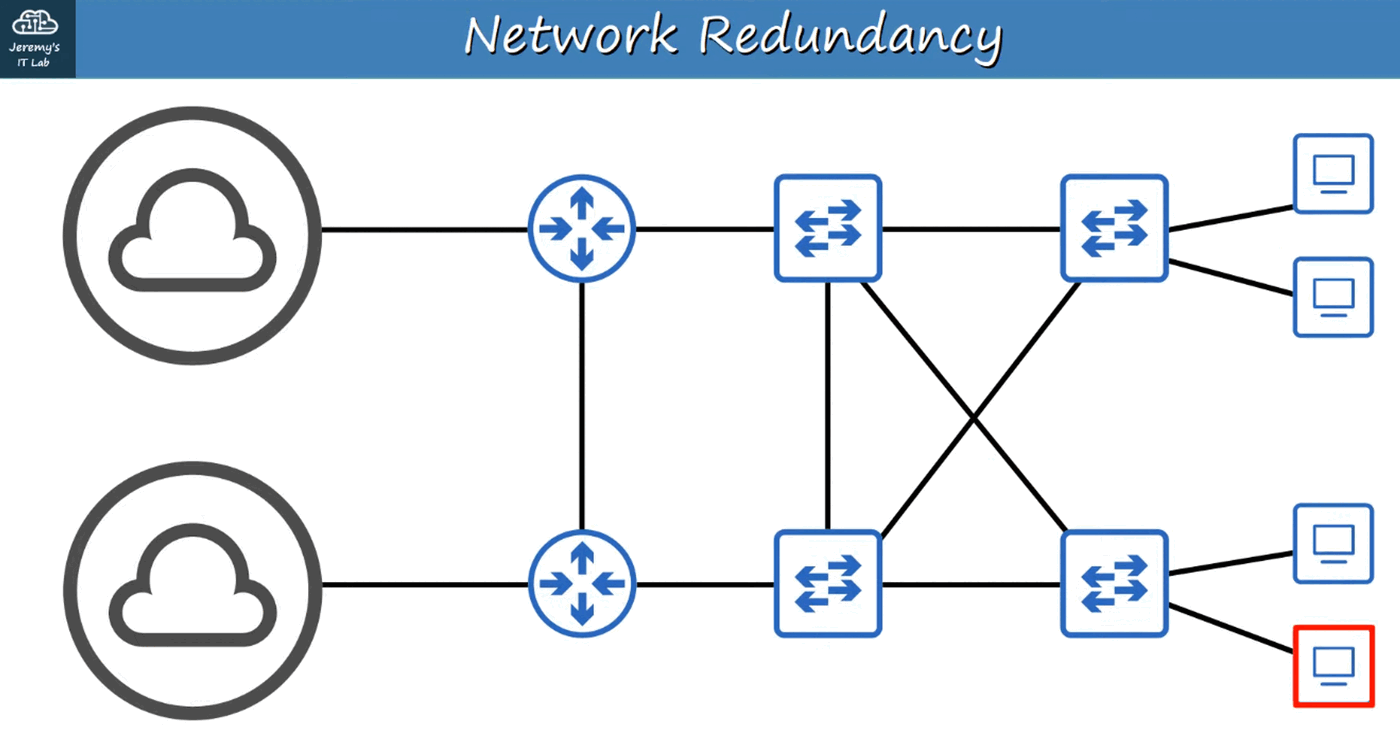
\includegraphics[keepaspectratio,alt={image}]{images/21-spanning-tree-protocol-part1/img-002.png}}
\end{figure}

\section{Unfortunately}\label{unfortunately}

\begin{itemize}
\tightlist
\item
  Most PCS only have a single network interface card (NIC), so they can
  only be plugged into a single SWITCH. However, important SERVERS
  typically have multiple NICs, so they can be plugged into multiple
  SWITCHES for redundancy!
\end{itemize}

So HOW can all this redundancy be a BAD thing?

\section{Broadcast Storms}\label{broadcast-storms}

\begin{figure}
\centering
\pandocbounded{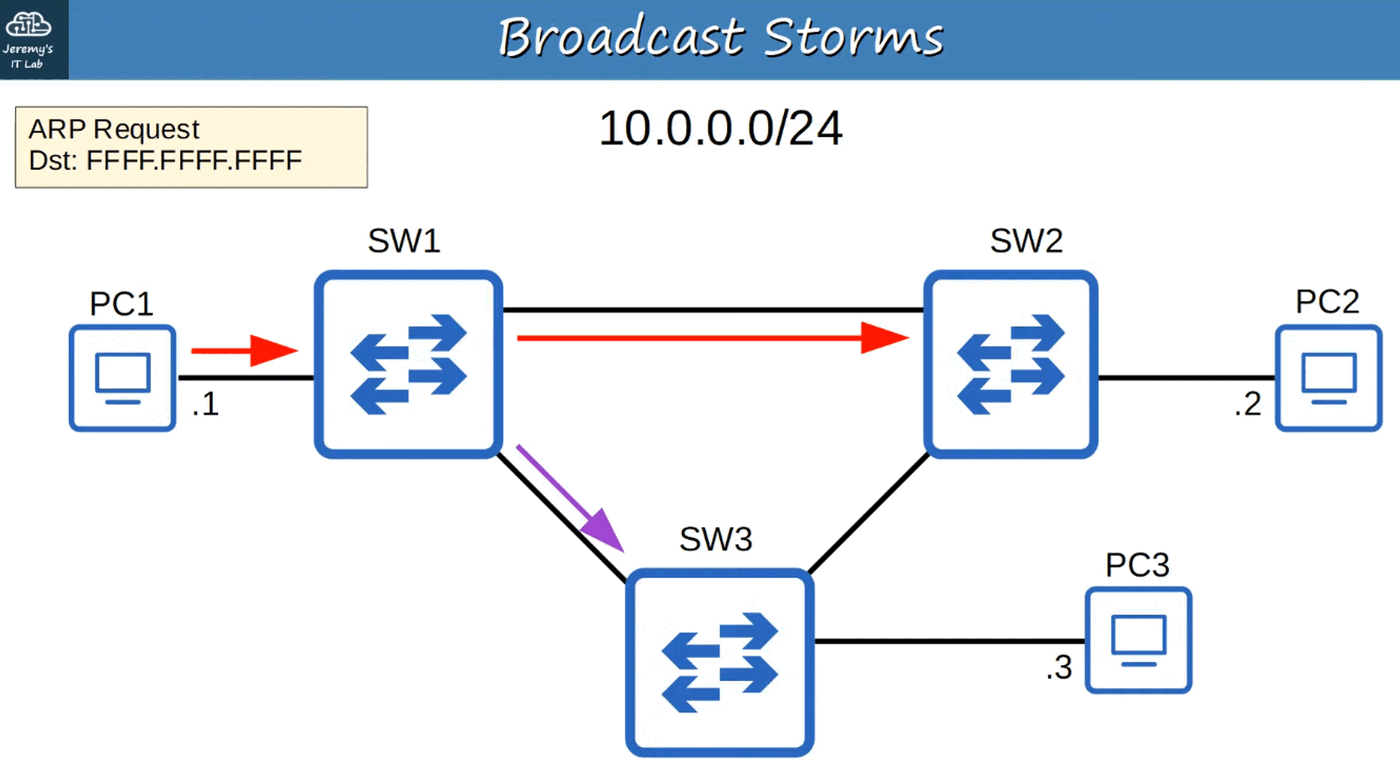
\includegraphics[keepaspectratio,alt={image}]{images/21-spanning-tree-protocol-part1/img-003.png}}
\end{figure}

\begin{figure}
\centering
\pandocbounded{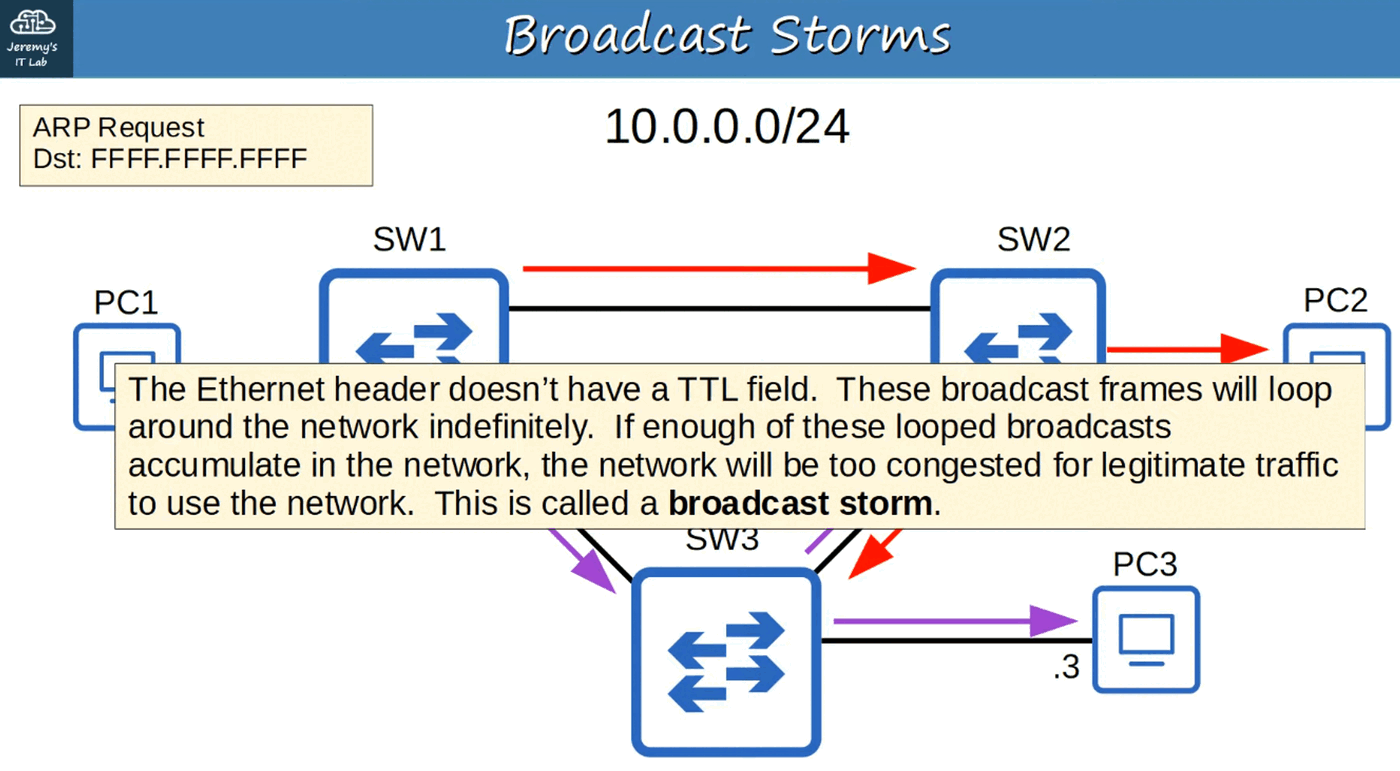
\includegraphics[keepaspectratio,alt={image}]{images/21-spanning-tree-protocol-part1/img-004.png}}
\end{figure}

\begin{figure}
\centering
\pandocbounded{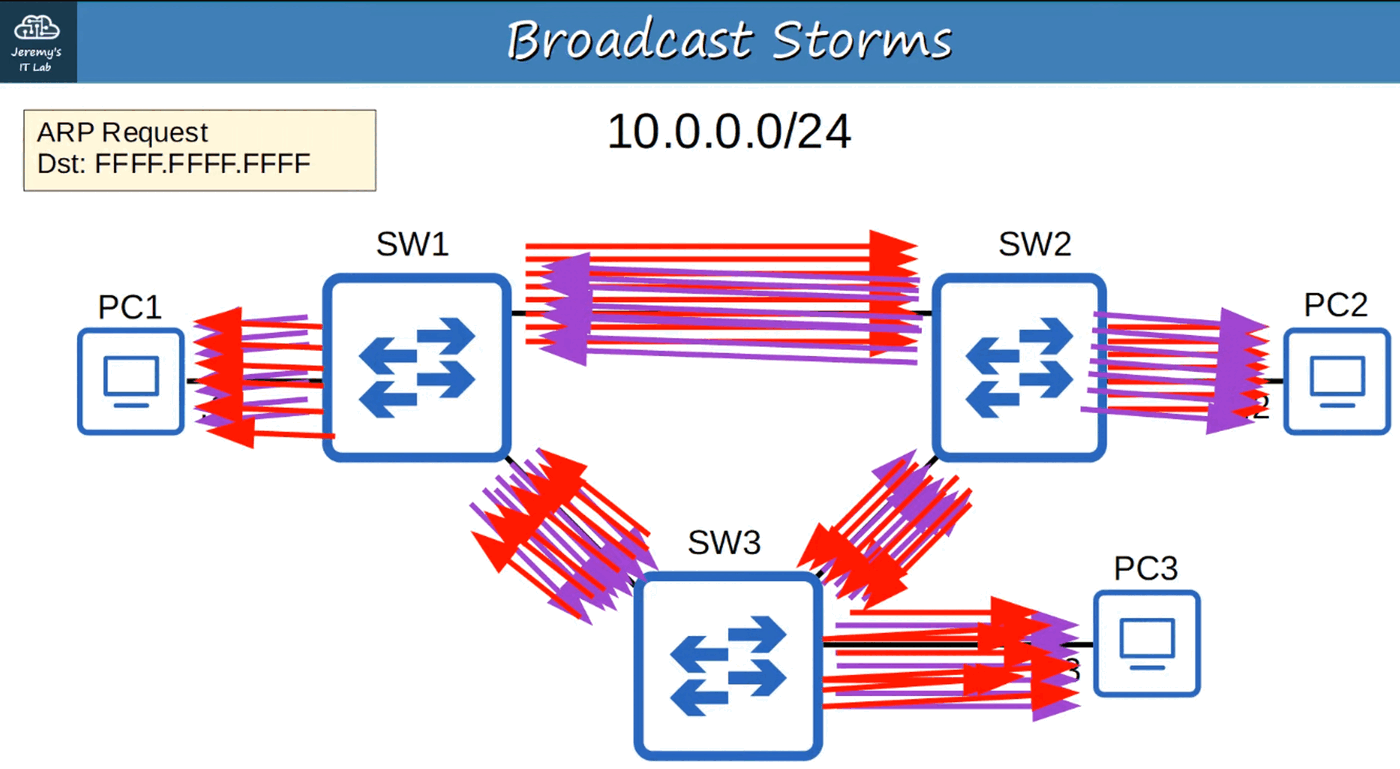
\includegraphics[keepaspectratio,alt={image}]{images/21-spanning-tree-protocol-part1/img-005.png}}
\end{figure}

FLOODED WITH ARP REQUESTS (Red = Clockwise Loops // Purple =
Counter-Clockwise Loops)

Network Congestion isn't the only problem.

Each time a FRAME arrives on a SWITCHPORT, the SWITCH uses the SOURCE
MAC ADDRESS field to ``learn'' the MAC ADDRESS and update it's MAC
ADDRESS TABLE.

When frames with the same SOURCE MAC ADDRESS repeatedly arrive on
different interfaces, the SWITCH is continuously updating the interface
in it's MAC ADDRESS TABLE.

This is called MAC ADDRESS FLAPPING

So how we design a network, with redundant paths, that doesn't result in
LAYER 2 LOOPS.

SPANNING TREE PROTOCOL is one solution

\section{STP (Spanning Tree Protocol) :
802.1D}\label{stp-spanning-tree-protocol-802.1d}

\begin{itemize}
\tightlist
\item
  ``Classic Spanning Tree Protocol'' is IEEE \textbf{802.1D}
\item
  SWITCHES from ALL vendors run STP by Default
\item
  STP prevents LAYER 2 loops by placing redundant PORTS in a BLOCKING
  state, essentially disabling the INTERFACE
\item
  These INTERFACES act as backups that can enter a FORWARDING state if
  an active (=currently forwarding) INTERFACE fails.
\item
  INTERFACES in a BLOCKING state only send or receive STP messages
  (called BPDUs = Bridge Protocol Data Units)
\end{itemize}

SPANNING TREE PROTOCOL still uses the term ``BRIDGE''. However, when use
the term ``BRIDGE'', we really mean ``SWITCH''. BRIDGES are not used in
modern networks.

\begin{figure}
\centering
\pandocbounded{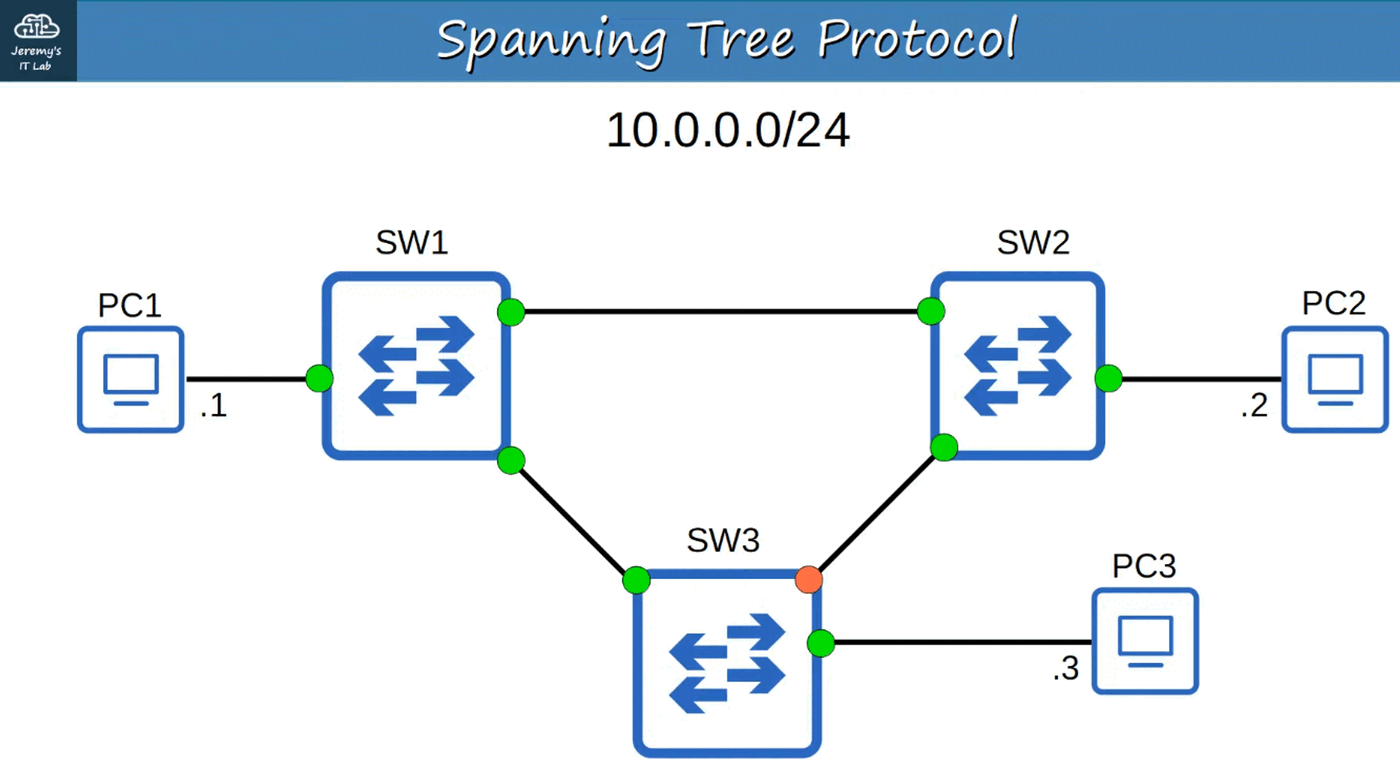
\includegraphics[keepaspectratio,alt={image}]{images/21-spanning-tree-protocol-part1/img-006.png}}
\end{figure}

ORANGE INTERFACE is ``BLOCKED'' causing a break in the loops

\begin{figure}
\centering
\pandocbounded{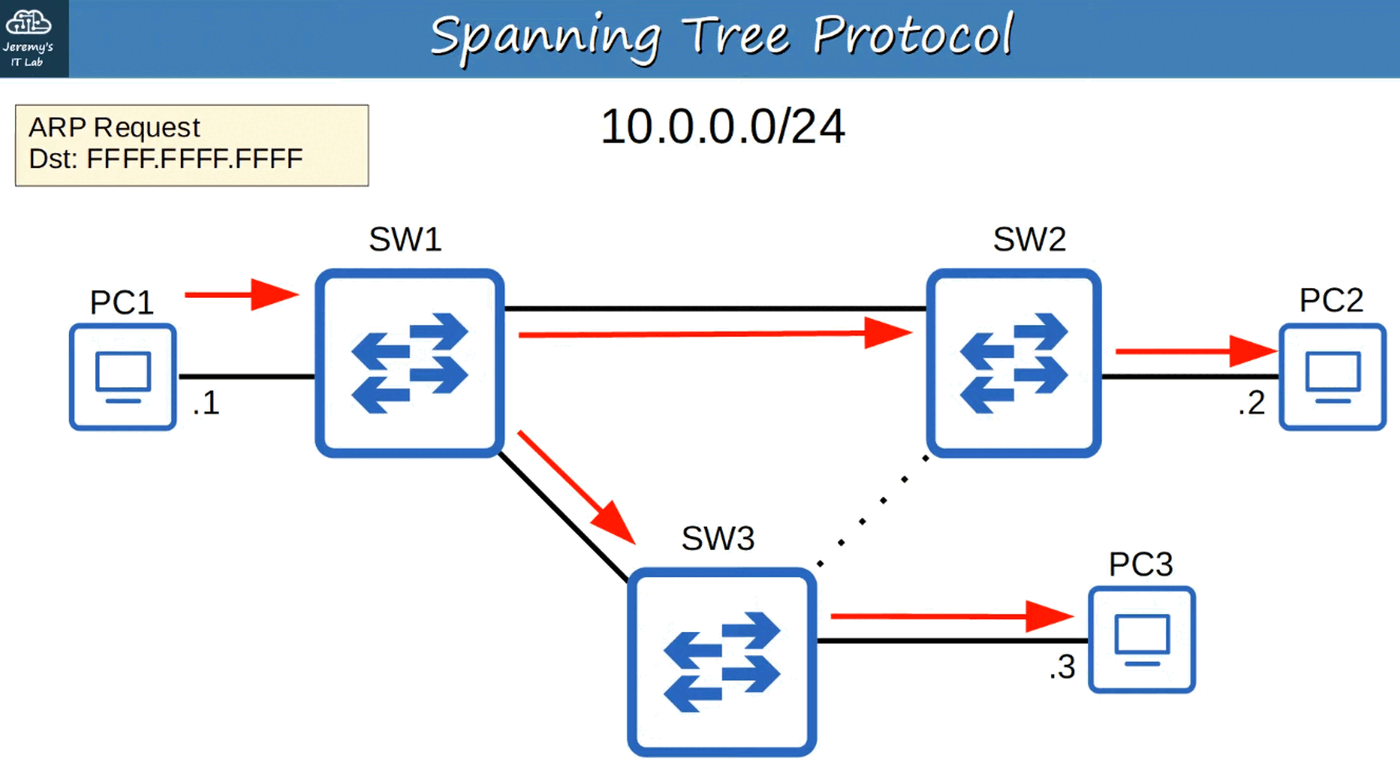
\includegraphics[keepaspectratio,alt={image}]{images/21-spanning-tree-protocol-part1/img-007.png}}
\end{figure}

If changes occur in the connections, the traffic will adjust the
topology.

\begin{itemize}
\tightlist
\item
  By selecting WHICH ports are FORWARDING and which ports are BLOCKING,
  STP creates a single path TO / FROM each point in the NETWORK. This
  prevents LAYER 2 Loops.
\item
  There is a set process that STP uses to determine which ports should
  be FORWARDING and which should be BLOCKING
\item
  STP-enabled SWITCHES send / receive ``Hello BPDUs'' out of all
  INTERFACES

  \begin{itemize}
  \tightlist
  \item
    The default timer is : ONCE every TWO seconds per INTERFACE!
  \end{itemize}
\item
  If a SWITCH receives a ``Hello BPDU'' on an INTERFACE, it knows that
  INTERFACE is connected to another SWITCH (ROUTERS, PCs, etc. do NOT
  use STP so do not send ``Hello BPDUs'')
\end{itemize}

WHAT ARE BPDUs USED FOR?

\begin{itemize}
\tightlist
\item
  SWITCHES use one field in the STP BPDU, the BRIDGE ID field, to elect
  a ROOT BRIDGE for the NETWORK
\item
  The SWITCH with the lowest BRIDGE ID becomes the ROOT BRIDGE
\item
  ALL PORTS on the ROOT BRIDGE are put in a FORWARDING state, and other
  SWITCHES in the topology must have a path to reach the ROOT BRIDGE
\end{itemize}

\begin{figure}
\centering
\pandocbounded{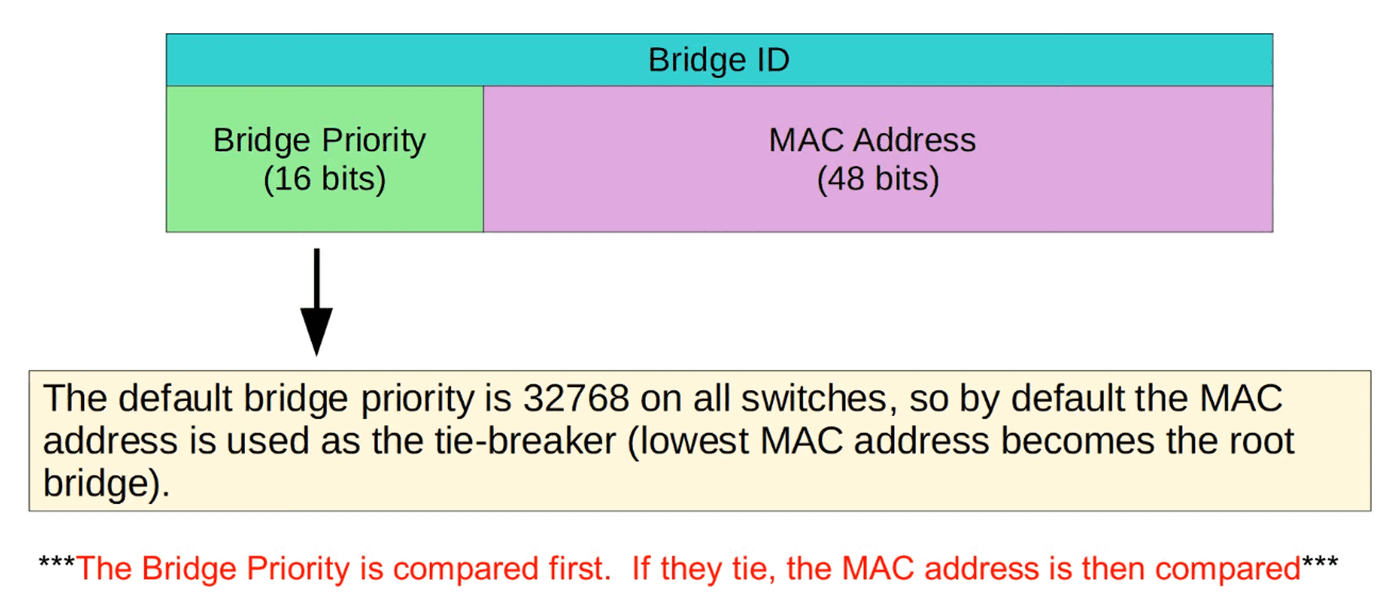
\includegraphics[keepaspectratio,alt={image}]{images/21-spanning-tree-protocol-part1/img-008.png}}
\end{figure}

\begin{figure}
\centering
\pandocbounded{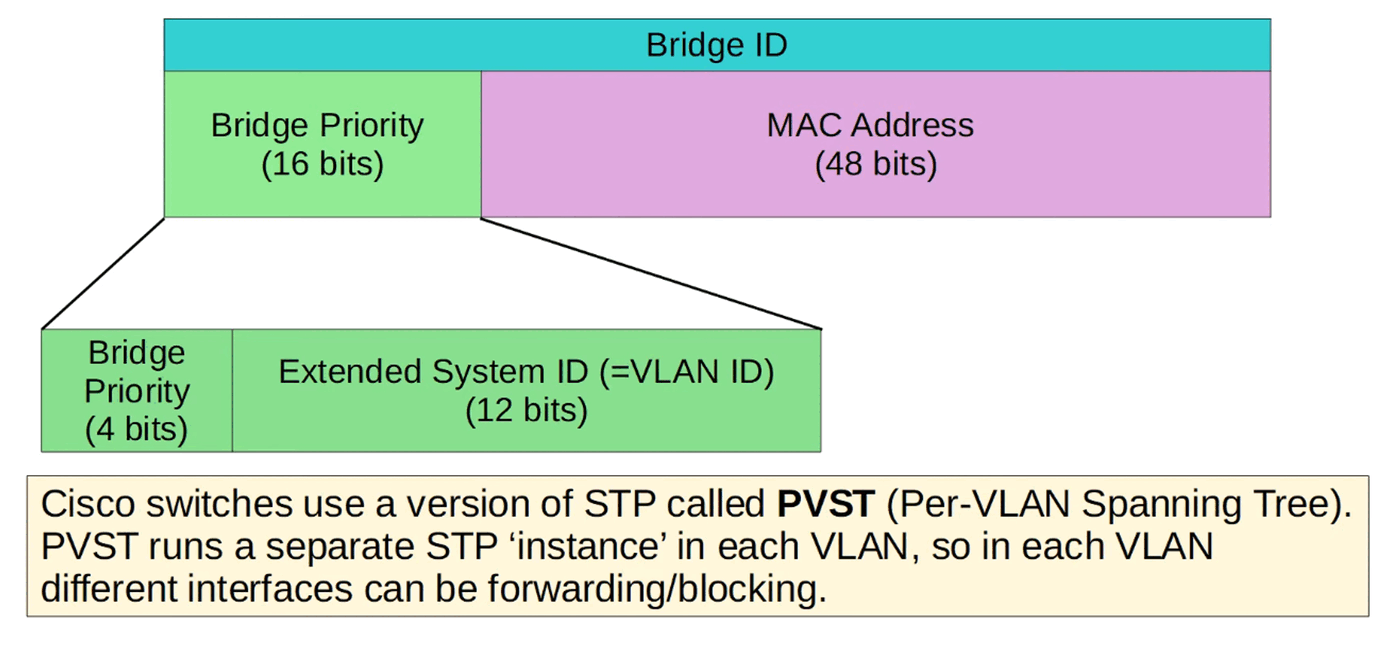
\includegraphics[keepaspectratio,alt={image}]{images/21-spanning-tree-protocol-part1/img-009.png}}
\end{figure}

\begin{figure}
\centering
\pandocbounded{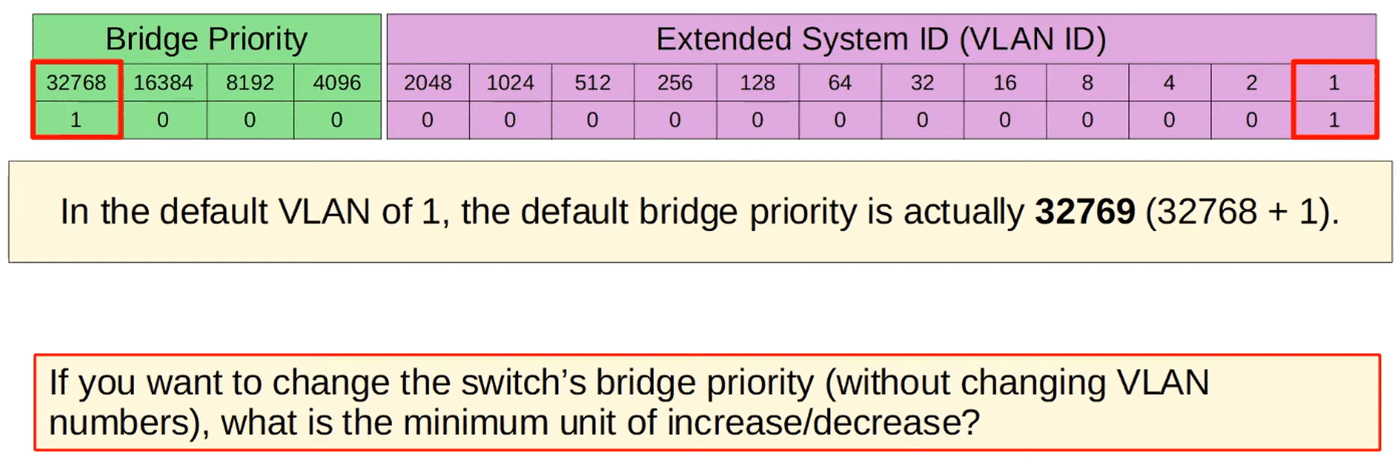
\includegraphics[keepaspectratio,alt={image}]{images/21-spanning-tree-protocol-part1/img-010.png}}
\end{figure}

To REDUCE the BRIDGE PRIORITY, we can only change it in units of 4096 !

\begin{figure}
\centering
\pandocbounded{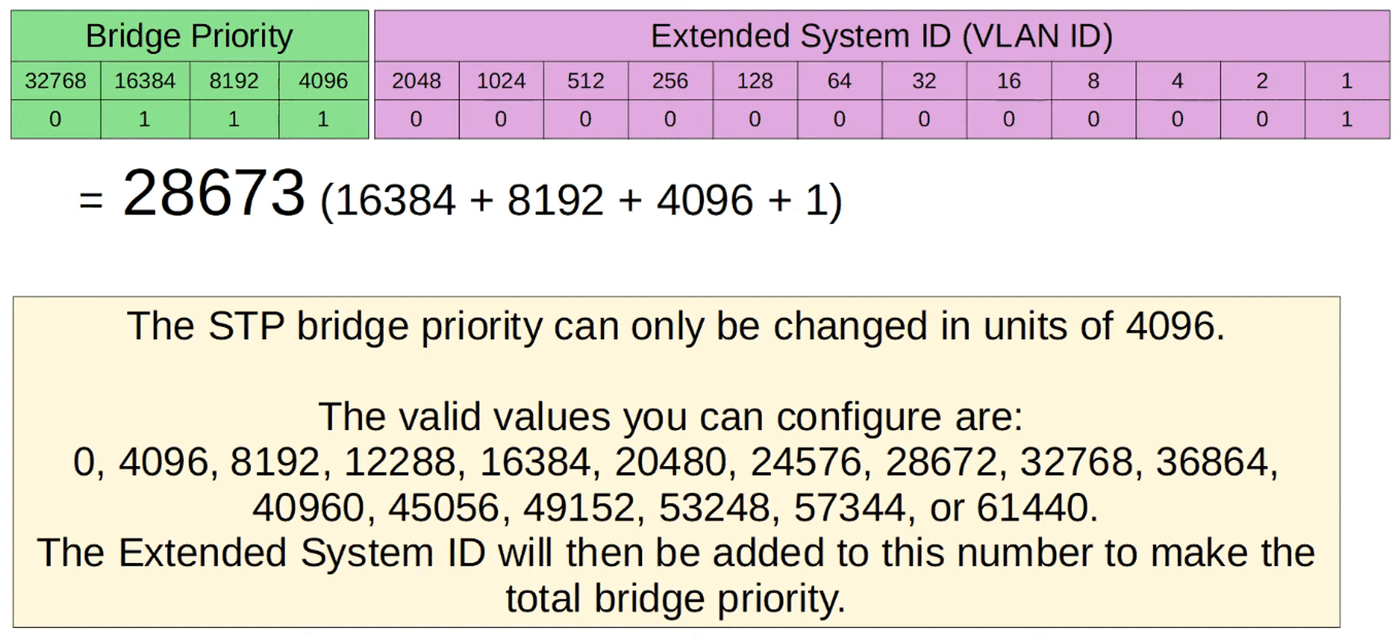
\includegraphics[keepaspectratio,alt={image}]{images/21-spanning-tree-protocol-part1/img-011.png}}
\end{figure}

In THIS TOPOLOGY, SW1 becomes the ROOT BRIDGE due to it's MAC ADDRESS
being LOWEST

(Hex ``A'' = 10)

\begin{figure}
\centering
\pandocbounded{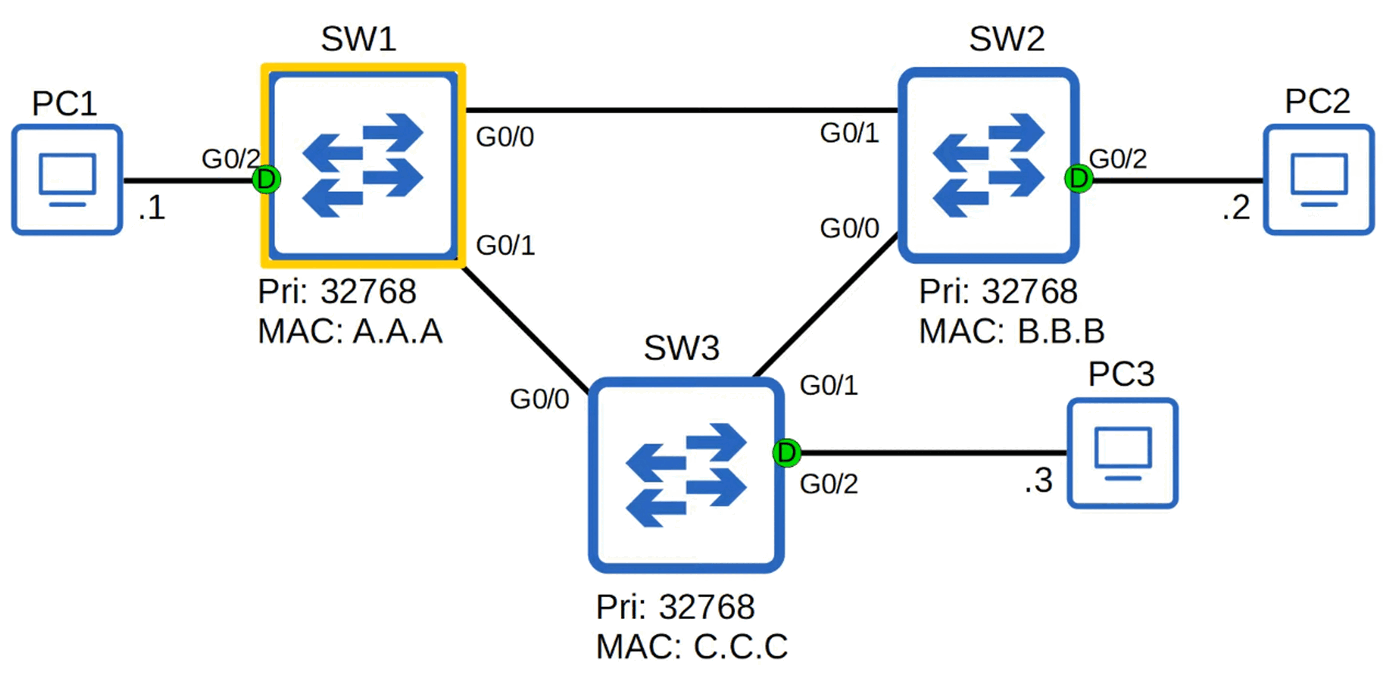
\includegraphics[keepaspectratio,alt={image}]{images/21-spanning-tree-protocol-part1/img-012.png}}
\end{figure}

ALL INTERFACES on the ROOT BRIDGE are DESIGNATED PORTS.

DESIGNATED PORTS ARE IN A FORWARDING STATE!

\section{Root Bridge}\label{root-bridge}

\begin{itemize}
\tightlist
\item
  When a SWITCH is powered on, it assumes it is the ROOT BRIDGE
\item
  It will only give up its position if it receives a ``SUPERIOR'' BPDU
  (lower BRIDGE ID)
\item
  Once the topology has converged and all SWITCHES agree on the ROOT
  BRIDGE, only the ROOT BRIDGE sends BPDUs
\item
  Other SWITCHES in the network will forward these BPDUs, but will not
  generate their own original BPDUs
\end{itemize}

\section{Spanning Tree Protocol
Steps}\label{spanning-tree-protocol-steps}

\begin{enumerate}
\def\labelenumi{\arabic{enumi})}
\tightlist
\item
  One SWITCH is elected as ROOT BRIDGE. All PORTS on the ROOT BRIDGE are
  DESIGNATED PORTS (FORWARDING STATE)
\end{enumerate}

\begin{itemize}
\tightlist
\item
  ROOT BRIDGE selection order:

  \begin{itemize}
  \tightlist
  \item
    \begin{enumerate}
    \def\labelenumi{\arabic{enumi})}
    \tightlist
    \item
      Lowest BRIDGE ID
    \end{enumerate}
  \item
    2) Lowest MAC Address (in case of Bridge ID tie)
  \end{itemize}
\end{itemize}

\begin{enumerate}
\def\labelenumi{\arabic{enumi})}
\setcounter{enumi}{1}
\tightlist
\item
  Each remaining SWITCH will select ONE of its INTERFACES to be it's
  ROOT PORT (FORWARDING STATE). PORTS across from the ROOT PORT are
  always DESIGNATED PORTS.
\end{enumerate}

\begin{itemize}
\tightlist
\item
  ROOT PORT selection order:

  \begin{itemize}
  \tightlist
  \item
    \begin{enumerate}
    \def\labelenumi{\arabic{enumi})}
    \tightlist
    \item
      LOWEST ROOT COST (see STP COST CHART)
    \end{enumerate}
  \item
    2) LOWEST NEIGHBOUR BRIDGE ID
  \item
    3) LOWEST NEIGHBOUR PORT ID
  \end{itemize}
\end{itemize}

\begin{enumerate}
\def\labelenumi{\arabic{enumi})}
\setcounter{enumi}{2}
\tightlist
\item
  Each remaining COLLISION DOMAIN will select ONE INTERFACE to be a
  DESIGNATION PORT (FORWARDING STATE). The other PORT in the COLLISION
  DOMAIN will NON-DESIGNATED (BLOCKING)
\end{enumerate}

\begin{itemize}
\tightlist
\item
  DESIGNATED PORT SELECTION:

  \begin{itemize}
  \tightlist
  \item
    \begin{enumerate}
    \def\labelenumi{\arabic{enumi})}
    \tightlist
    \item
      INTERFACE on SWITCH with LOWEST ROOT COST
    \end{enumerate}
  \item
    2) INTERFACE on SWITCH with LOWEST BRIDGE ID
  \end{itemize}
\end{itemize}

\section{STP Cost Chart}\label{stp-cost-chart}

Only OUTGOING INTERFACES toward the ROOT BRIDGE have a STP COST; not
RECEIVING INTERFACES. Add up all the OUTGOING PORT costs until you reach
the ROOT BRIDGE

\begin{figure}
\centering
\pandocbounded{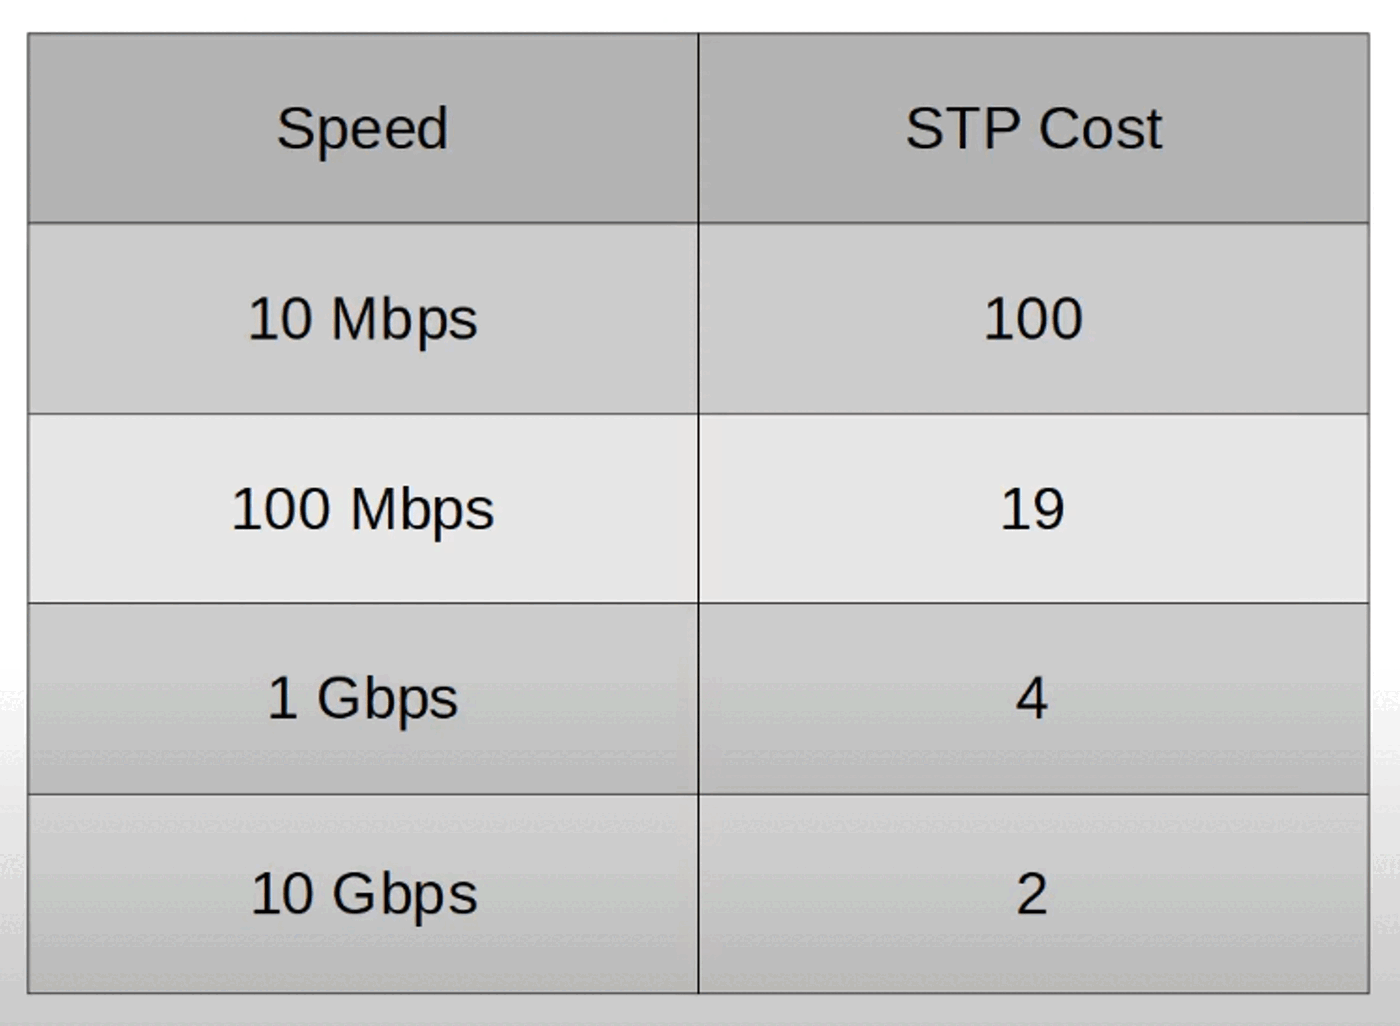
\includegraphics[keepaspectratio,alt={image}]{images/21-spanning-tree-protocol-part1/img-013.png}}
\end{figure}

SW1 is the ROOT BRIDGE so has a STP COST of 0 on ALL INTERFACES

\begin{figure}
\centering
\pandocbounded{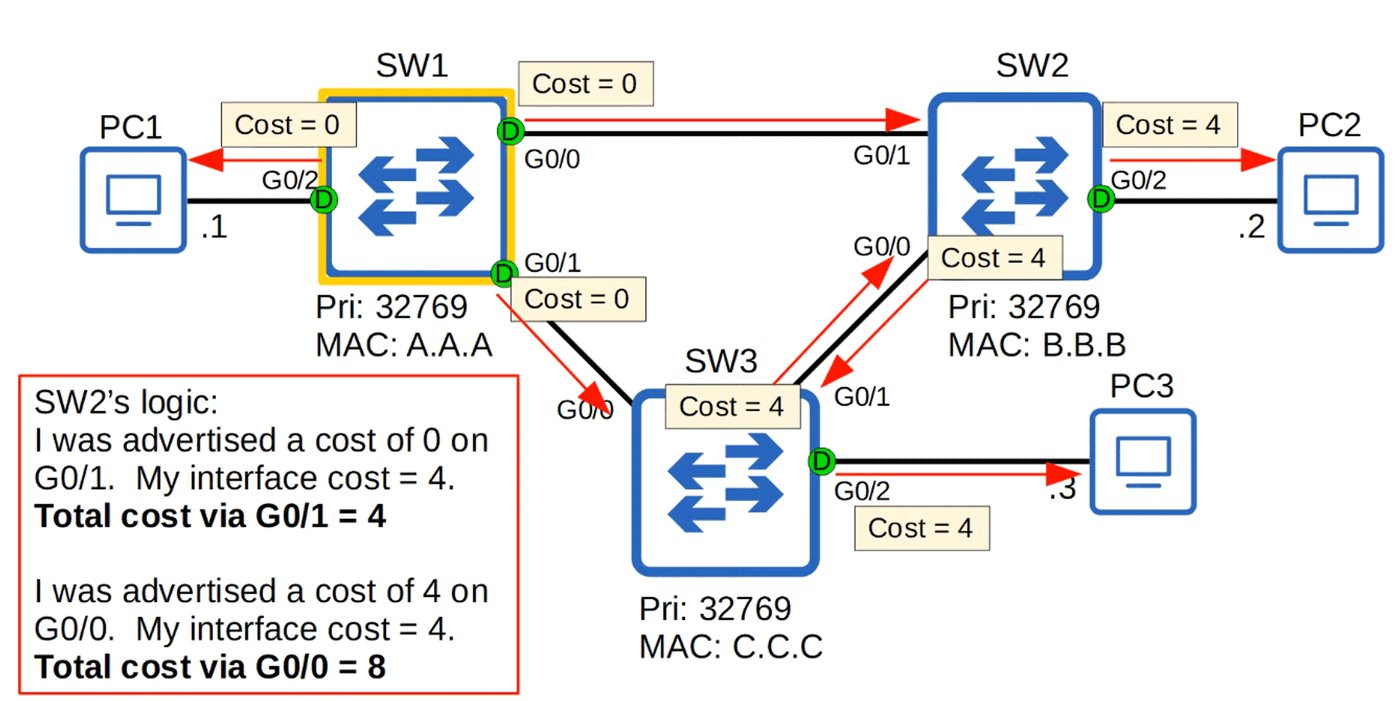
\includegraphics[keepaspectratio,alt={image}]{images/21-spanning-tree-protocol-part1/img-014.png}}
\end{figure}

The PORTS connected to another SWITCH's ROOT PORT MUST be DESIGNATED
(D).

Because the ROOT PORT Is the SWITCH's path to the ROOT BRIDGE, another
SWITCH must not block it.

STP PORT ID (in case of a tie-breaker)

\begin{figure}
\centering
\pandocbounded{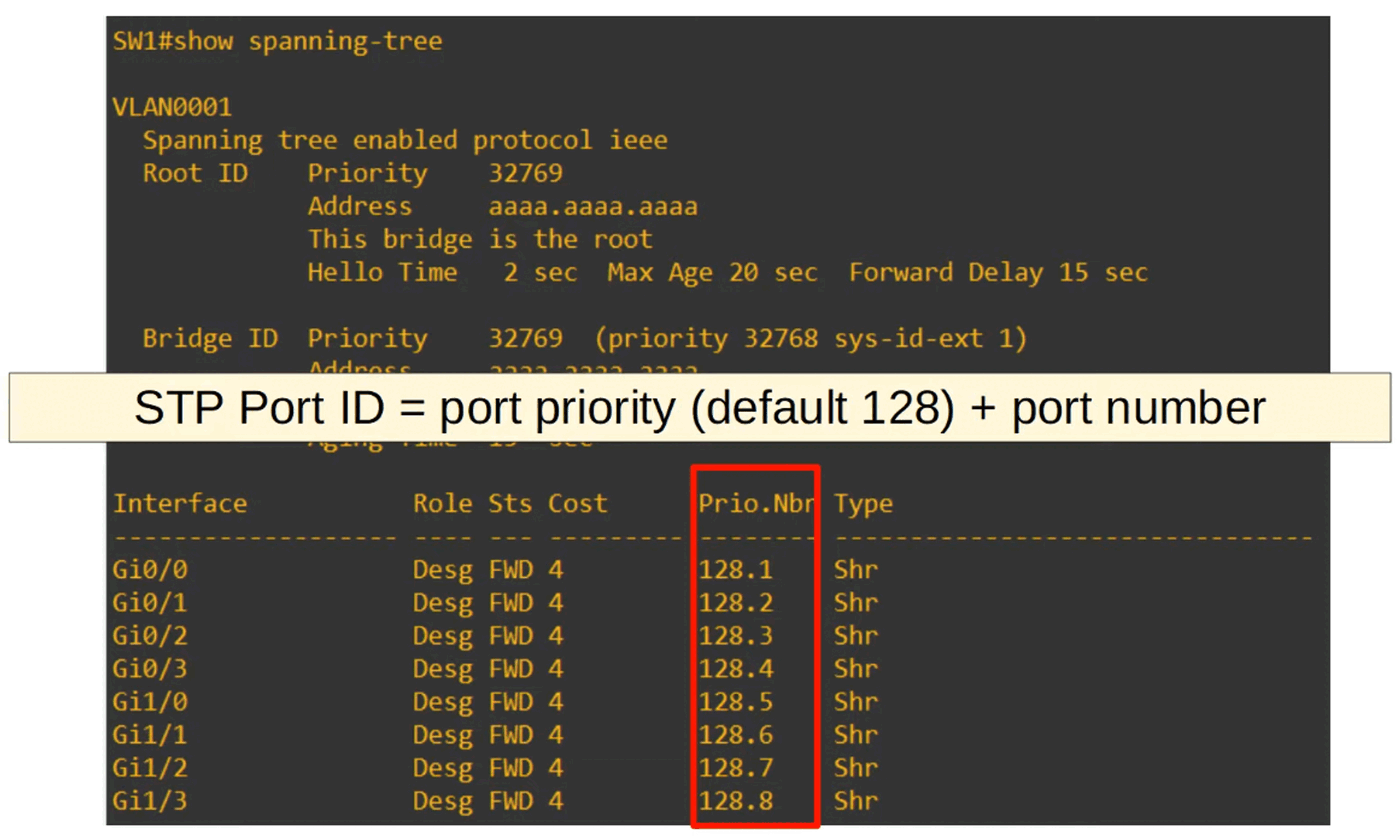
\includegraphics[keepaspectratio,alt={image}]{images/21-spanning-tree-protocol-part1/img-015.png}}
\end{figure}

NEIGHBOUR SWITCH PORT ID (in case of a tie-breaker)

\begin{enumerate}
\def\labelenumi{(\Alph{enumi})}
\setcounter{enumi}{3}
\item
  = DESIGNATED PORT
\item
  = ROOT PORT
\end{enumerate}

\begin{figure}
\centering
\pandocbounded{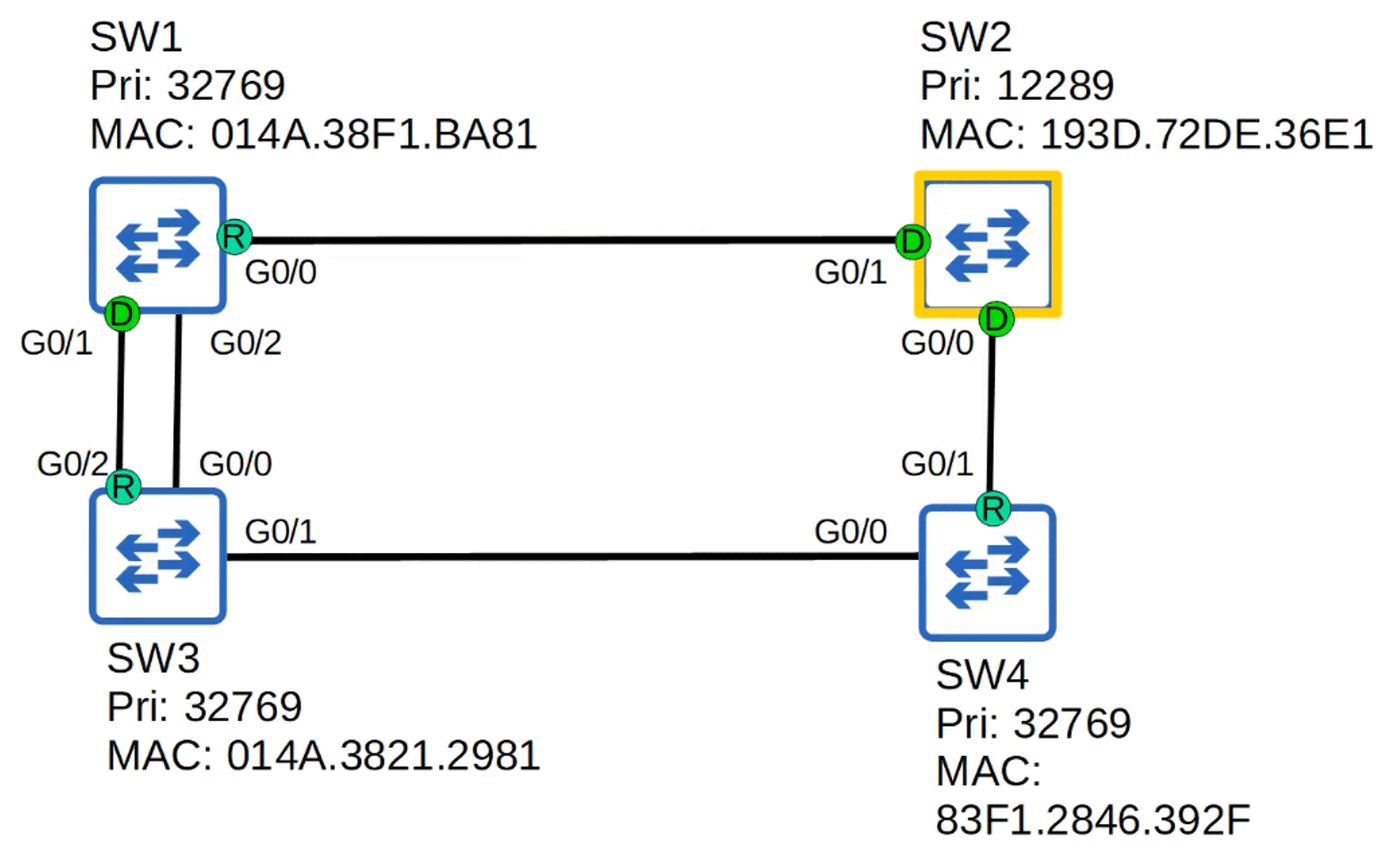
\includegraphics[keepaspectratio,alt={image}]{images/21-spanning-tree-protocol-part1/img-016.png}}
\end{figure}

\section{How to Determine Which Port Will Be Blocked to Prevent Layer 2
Loops}\label{how-to-determine-which-port-will-be-blocked-to-prevent-layer-2-loops}

\begin{figure}
\centering
\pandocbounded{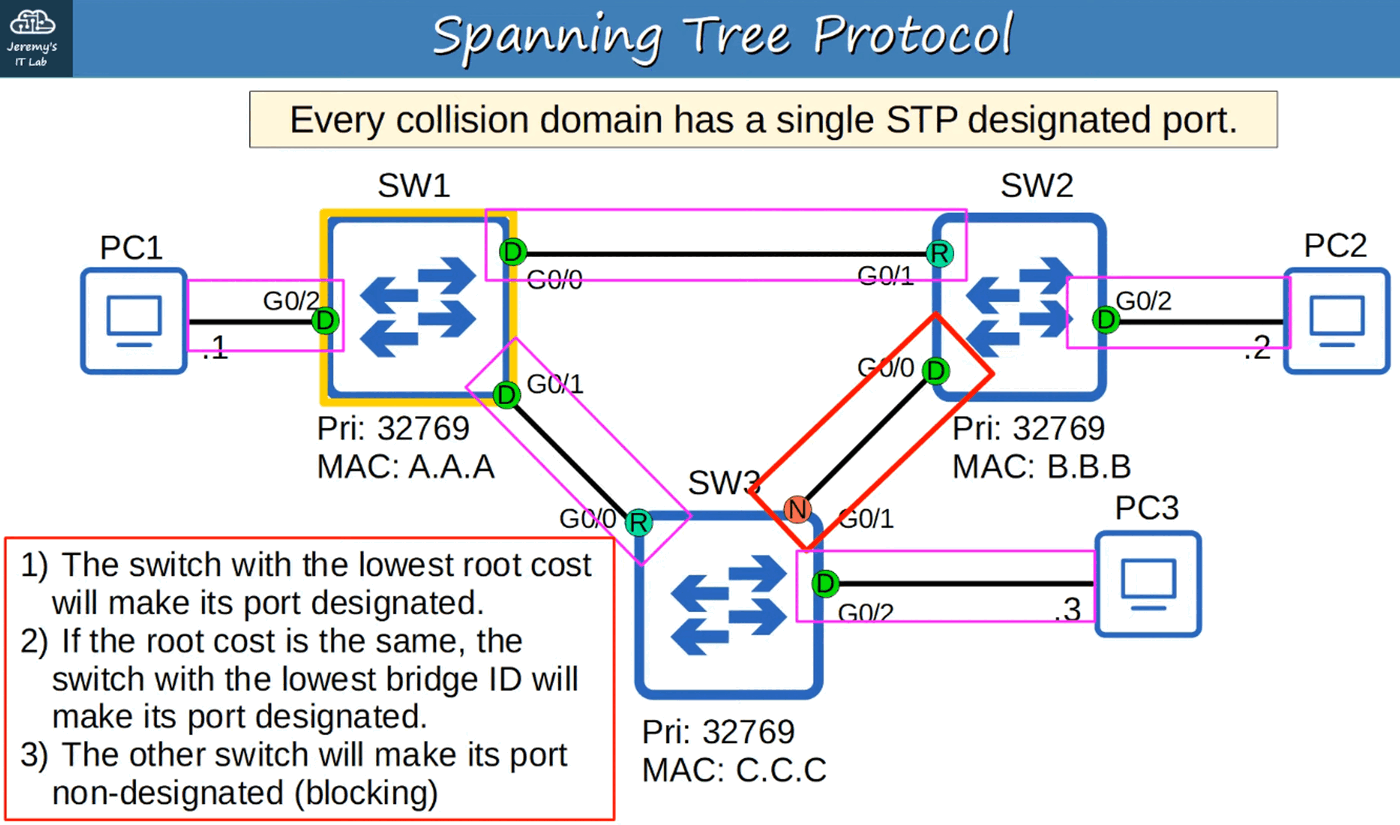
\includegraphics[keepaspectratio,alt={image}]{images/21-spanning-tree-protocol-part1/img-017.png}}
\end{figure}

\section{Quiz}\label{quiz}

Identify the ROOT BRIDGE and the ROLE of EACH INTERFACE on the NETWORK
(ROOT / DESIGNATED / NON-DESIGNATED)

\#1

\begin{figure}
\centering
\pandocbounded{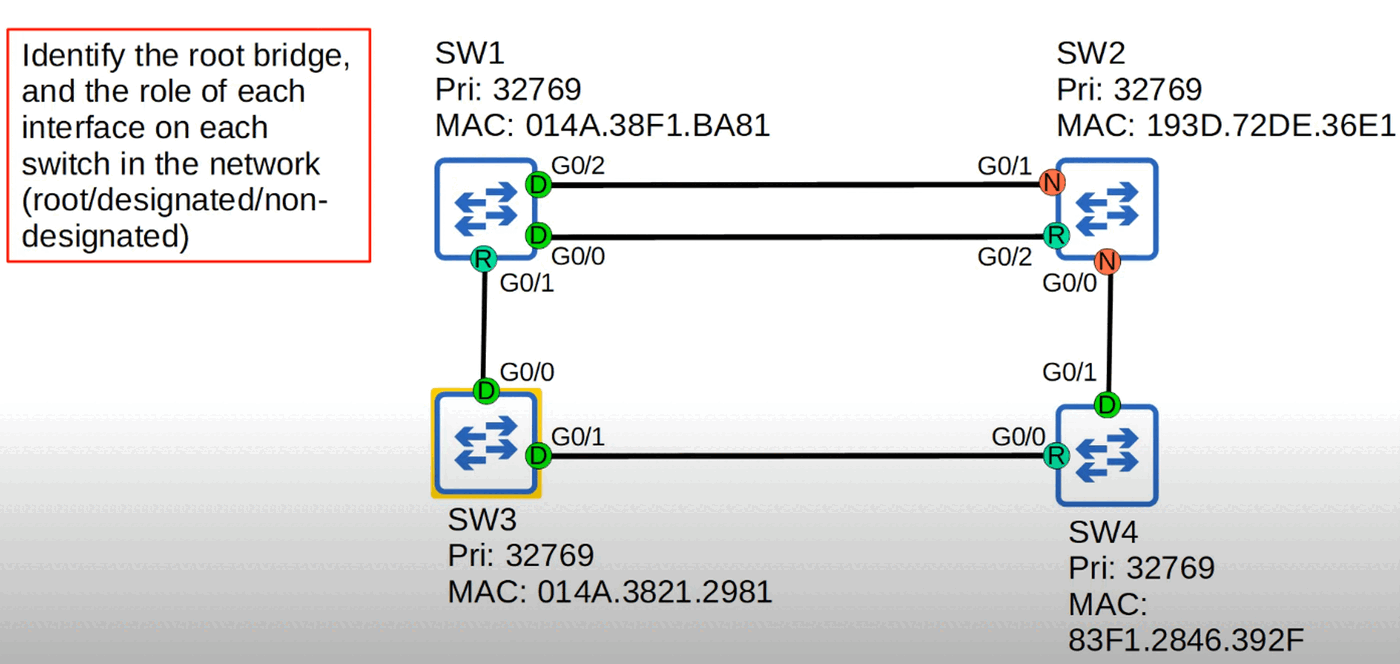
\includegraphics[keepaspectratio,alt={image}]{images/21-spanning-tree-protocol-part1/img-018.png}}
\end{figure}

ALL SWITCHES have the same PRIORITY NUMBER (32769)

Tie-breaker goes to the LOWEST MAC ADDRESS

SW3 has the LOWEST so it's the ROOT BRIDGE and ALL it's INTERFACES
become DESIGNATED

Connections from SW1 (G0/1) and S4 (G0/0) to SW3 become ROOT INTERFACES

Because SW2 has TWO connections to SW1, both of SW1's INCOMING
interfaces become DESIGNATED.

SW2 G0/2 INTERFACE becomes a ROOT INTERFACE because the G0/0 INTERFACE
of SW1 is LOWER than it's G0/2 INTERFACE

The remaining interfaces on SW2 become NON-DESIGNATED because it has the
HIGHEST ROOT COST (12 = 4x 1 GB connection). INTERFACES they are
attached to on other SWITCHES become DESIGNATED

\#2

\begin{figure}
\centering
\pandocbounded{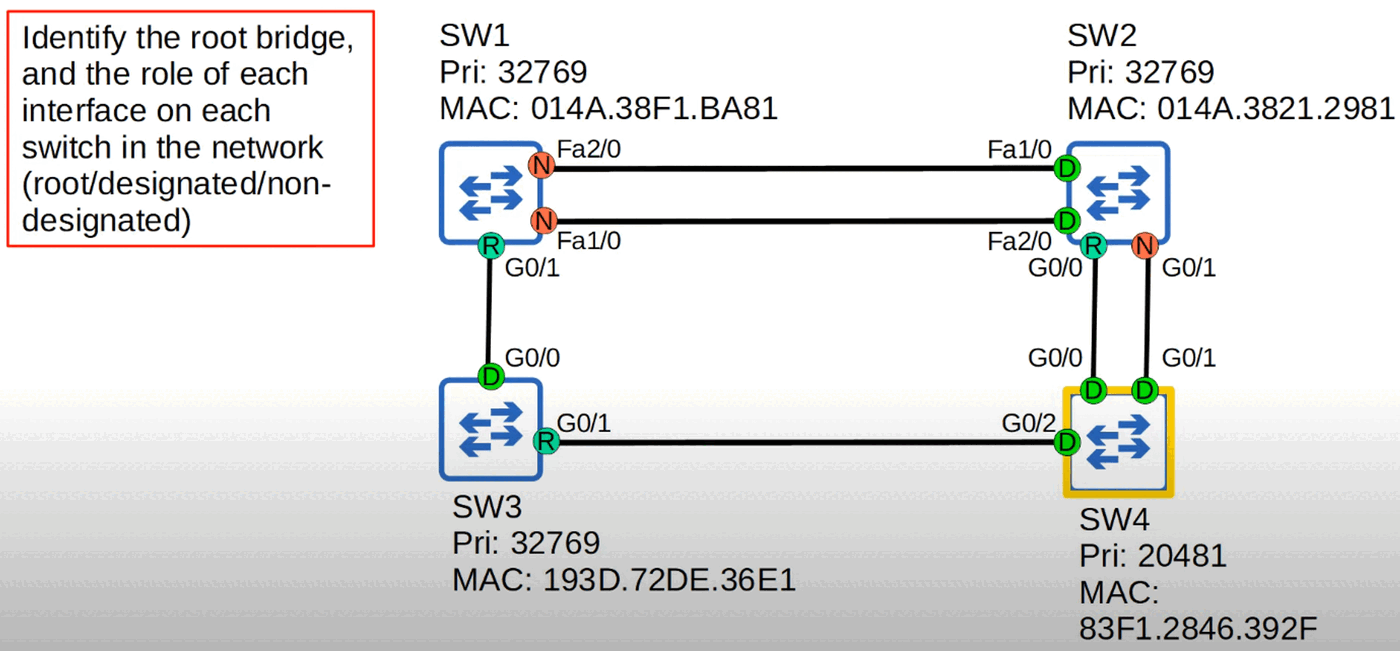
\includegraphics[keepaspectratio,alt={image}]{images/21-spanning-tree-protocol-part1/img-019.png}}
\end{figure}

SW4 has the LOWEST Priority Number so it is designated ROOT BRIDGE

All of SW4 INTERFACES become DESIGNATED

SW2 G0/0 becomes ROOT PORT because SW4 G0/0 connection is a LOWER NUMBER
than G0/1.

SW3 G0/1 becomes ROOT PORT

SW1 G0/1 becomes ROOT PORT because G0/1 cost is LESS than Fa1/0 and 2/0

EACH remaining PORT will be either DESIGNATED or NON-DESIGNATED

SW1 Fa1/0 and 2/0 become NON-DESIGNATED since they have a HIGHER STP
COST (38) than SW2 outbound ports (8) making SW2 Fa1/0 and 2/0
DESIGNATED

SW2 remaining connection, G0/1, NON-DESIGNATED
